\documentclass{article}
\usepackage[final]{nips_2017}
\usepackage[utf8]{inputenc} % allow utf-8 input
\usepackage[T1]{fontenc}    % use 8-bit T1 fonts
\usepackage{hyperref}       % hyperlinks
\usepackage{url}            % simple URL typesetting
\usepackage{booktabs}       % professional-quality tables
\usepackage{amsfonts}       % blackboard math symbols
\usepackage{nicefrac}       % compact symbols for 1/2, etc.
\usepackage{microtype}      % microtypography
\usepackage{graphicx}
\title{Seeing Stars: A Computer Vision-Centered Approach for Star Rating in the Hospitality Industry \\
(Computer Vision)}

\author{
  Bo Xian Ye \\
  Graduate School of Business\\
  Stanford University\\
  \texttt{bxye@stanford.edu} \\
  SUNet ID 05160610\\
  \And
  Gangwei Zhuo \\
  Graduate School of Business\\
  Stanford University \\
  \texttt{gzhuo@stanford.edu} \\
  SUNet ID 05589467\\
  \And
  Isha Bhatt \\
  Stanford Center for \\
  Professional Development \\
  Stanford University \\
  \texttt{ishakb@stanford.edu} \\
  %% \And
  %% Coauthor \\
  %% Affiliation \\
  %% Address \\
  %% \texttt{email} \\
  %% \And
  %% Coauthor \\
  %% Affiliation \\
  %% Address \\
  %% \texttt{email} \\
}

\begin{document}
% \nipsfinalcopy is no longer used

\begin{center}
\includegraphics[width=3cm, height=0.7cm]{CS230}
\end{center}

\maketitle

\section{Problem Description}	
With over 10 million hotels globally, there is a need for travel booking websites to provide accurate and reliable information to visitors. Star rating is most frequently used as a filtering criterion, but is unreliable given the absence of commonly accepted standards for star rating assignment. Manual human verification can be subjective and incurs high operating costs. Several major third-party distribution platforms, e.g., Booking.com, therefore let hotel owners self-report their own star ratings, with highly inconsistent results. [1]

\section{Objective}	
\par Our objective is to create a computer-vision-assisted machine learning model that can more accurately assign hotel star ratings using images and meta-data (e.g. pricing, facilities). This promises a cheaper and more objective methodology in assigning hotel star ratings.

\section{Literature Survey}
While some researchers have pioneered the use of machine learning to determine star ratings, existing methods have centered on the use of natural language processing and sentiment analysis of user reviews [2], [3]. However, there are several technical and business challenges associated with this methodology, including the widespread phenomenon of using counterfeit reviews to boost ratings [4], and the noisiness of online user reviews. 

Computer vision accompanied with meta-data promises an alternative and relatively unexplored approach to determine the star rating of hotels. While deep learning is now commonly applied to the categorization of hotel images [5], no major market player in the world has attempted to apply it to the rating of hotels.

\section{Challenges}
We anticipate the following challenges:
\begin{itemize}
    \item Low volume of image, content, or transaction data for some hotels. 
    \item Non-standard accommodations (e.g. hostels, villas, boats) are substantially different from standard hotels in appearance and facilities, and require dedicated models to address. 
    \item Official hotel images are typically digitally altered for aesthetic appeal. This may narrow visual differences between the images of different star-rated hotels.

\end{itemize}


\section{Dataset}
We will employ a dataset from China’s largest travel booking site, Trip.com, containing metadata on 800,000 standard hotels in China. From this, we will employ a sub-set of about 55,000 hotels whose star ratings have been manually verified by Trip.com’s operation team, for training and development. Image data will be scraped from the website and merged with the meta-data. We plan to use a 300 by 225 image resolution for training, which is close to the resolution used by ImageNet. The image data is pre-categorized into exterior view, common areas, rooms, bath, dining, entertainment facilities, business facilities, and hotel services. Each photo type category will likely contain about 100K images. The image data will be randomly split into a 90\% training set and 10\% development set.  

\section{ Learning Method }
We plan to employ Convolutional Neural Networks (CNN) to process image data, and a Deep Neural Network (DNN) to process meta-data, and combine the outputs from images and metadata at the last layer of the neural network. Since the categories of photo type substantially differ from each other, we will use separate CNNs to train and test each photo type. We will use softmax as the activation function and cross-entropy as the loss function. The proposed architecture is illustrated in \textbf{Figure 1}.

\begin{figure}[htp]
    \centering
    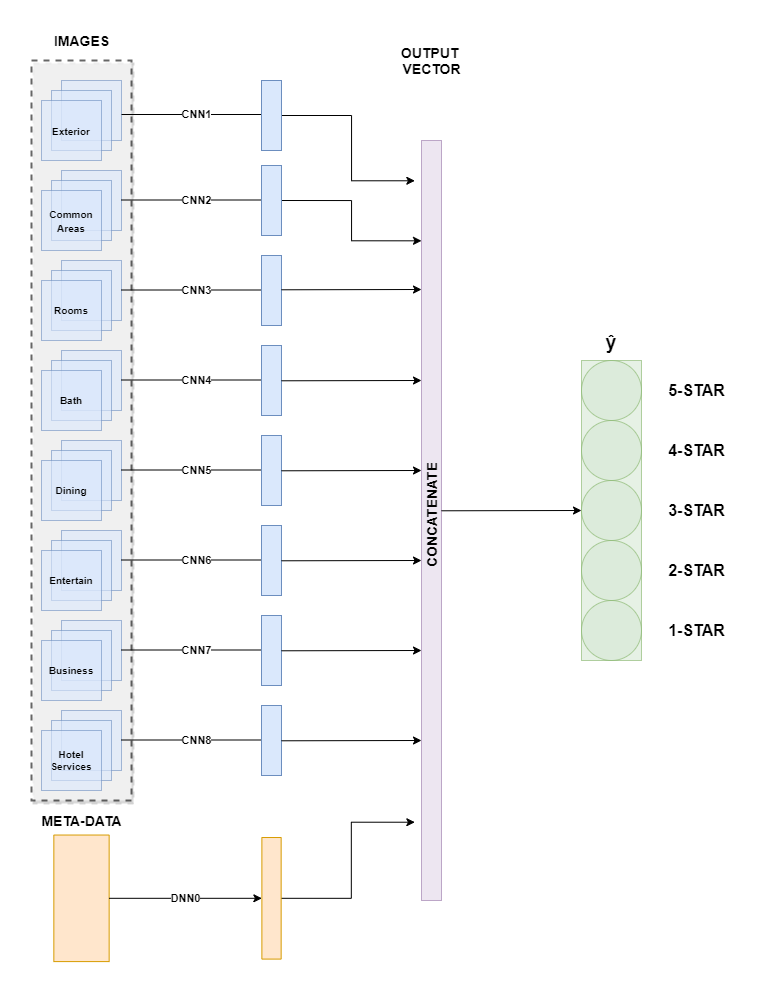
\includegraphics[width=14cm]{Architecture.png}
    \caption{Neural Network Architecture}
    \label{fig:architecture}
    \end{figure}

\section{Evaluation}
We aim to improve on several multi-class evaluation metrics including accuracy and F1 scores with the aid of computer vision. Earlier work by project collaborators employed a LASSO linear regression model to predict star ratings using structured hotel data without image data, achieving an accuracy of 68\%.\footnote{Accuracy is measured by number of prediction matching actual, divided by total number of hotels in development data set.} We also plan to compare the models' F1 scores since they can take into account class imbalance and can discriminate between different types of errors using the confusion matrix [6].\footnote{F1 score is found by taking the harmonic mean of the precision and recall, which are ratios computed from values in the confusion matrix. The macro-F1 score computes the per-class F1 scores and averages them and micro-F1 score aggregates the contributions of all classes to compute the final F1 score.} We will include a micro-F1 or a weighted macro-F1 score if there is a class imbalance in the examples across the five classes. 

\section*{References}
\medskip
\small
[1] Basak Denizci Guillet\ \& Rob Law\ (2010) Analyzing hotel star ratings on third‐party distribution websites. {\it International Journal of Contemporary Hospitality Management}.

[2] Shruthi, C G\ \& Gowrishankar, S.\ (2018) Machine Learning Based Comprehensive Analysis of Hospitality Industry in the State of Karnataka. {\it International Journal of Applied Engineering Research}.

[3] Kumar, B.Shiv,\ (2021) Predicting the ratings of reviews of a hotel using Machine Learning. \href{https://medium.com/analytics-vidhya/predicting-the-ratings-of-reviews-of-a-hotel-using-machine-learning-bd756e6a9b9b}{https://medium.com/analytics-vidhya/predicting-the-ratings-of-reviews-of-a-hotel-using-machine-learning-bd756e6a9b9b}.

[4] Pankaj Chaudhary,\ \ Dr Anurag Aeron\ \& Dr Sandeep Vijay\ (2019) Machine Learning as A Tool for Analysing Hotel Online Reviews. {\it International Journal of Engineering Research & Technology}.

[5] Trideep Rath\ \ (2018) Hotel Image Categorization with Deep Learning. \href{https://medium.com/kayak-tech/hotel-image-categorization-with-deep-learning-ffa8429e55b5}{https://medium.com/kayak-tech/hotel-image-categorization-with-deep-learning-ffa8429e55b5}.

[6] Margherita Grandini \ \& Enrico Bagli \ \& Giorgio Visani\ (2020) Metrics for Multi-Class Classification: An Overview.

\end{document}